\documentclass{article}
\usepackage{tikz}
%-----------------------
% Document information
%-----------------------


\title{Statistic Stuffs}

\author{Roberto \textsc{Antoniello}}

\begin{document}

\maketitle

\begin{center} I will drop here some statistic concepts I liked during the course I had at University of Milan.\end{center}

\section{Gini index}

There are two types of Gini indexes. One has the purpose of telling how much a sample is heterogeneous. The other one is used for concentration. We will talk about the first one we have mentioned and it's defined as follow:
\begin{center}$$I = 1 - \sum_{j=1}^{k}f_j^2$$\end{center}

This index is always less than 1 and it's always more than 0.

\begin{center}$0 \leq I < 1$\end{center}

So we are subtracting the squared relative frequencies from one. 

we know that: 
\begin{center}$$\forall j f_j \ge 0 \longrightarrow \sum_{j=1}^k f_j = 1$$.\end{center}

This implies that $\exists \acute{j} : \acute{f_j} > 0 \longrightarrow f_j^2 > 0$.

So: \begin{center}$$\sum_{j=1}^k f_j^2 > 0 \longrightarrow I < 1$$ as said in before.\end{center}

We can consider also that: $$\sum_{j=1}^kf_j^2 \le \sum_{j=1}^kf_j$$.

This implies that $$1 - \sum_{j=1}^kf_j^2 \ge 0$$.

We have just demonstrated what we said a few moments ago. $0 \leq I < 1$.  

\section{Probability calculus}

Before we can talk about probability, we have to define a probability function. So we need to define as first $\Omega$ as the set of all possibles outcomes. Then we can say what is an event, which is just a subset of $\Omega$. Now let's define what is an Event algebra:
$$\mathcal{A} = \left\{E_i \subseteq \Omega\right\}$$
$E_i$ are all the subsets events in $\Omega$. This algebra has to respect three rules:

1. $\Omega \in \mathcal{A}$

2. $\forall E \subseteq \Omega \longrightarrow E \in \Omega \rightarrow \bar E \in \Omega$

3. $\forall E,F \subseteq \Omega \longrightarrow E \in \mathcal{A}, F \in \mathcal{A} \rightarrow E \cup F \in \mathcal{A}$

The third rule can be extended to this: $$\forall i=1,2,..,n E_i \subseteq \Omega, E_i \in \mathcal{A} \rightarrow \bigcup_{i=1}^nE_i \in \mathcal{A}$$

Finally we can define the probability function.

$P  :  \mathcal{A} \rightarrow \mathbb{R}$

\subsection{Kolmogorov axioms}

Kolmogorov axioms are the fundamental rules of the probability calculus.

A1. $\forall E \in \mathcal{A} \ \ 0 \leq P(E) \leq 1$

A2. $P(\Omega) = 1$

A3. $\forall E_1...E_n \ \ \forall i \ E_i \in \mathcal{A}$ mutually exclusive $\rightarrow P(\bigcup_{i=1}^nE_i) = \sum_{i=1}^nP(E_i)$

\subsection{Elemental theorems of Probability}

1. First theorem

$\forall E \in \mathcal{A} \ \ \ P(\bar E) = 1 - P(E)$
\bigskip

Demonstration:

We know that $1 = P(\Omega)$ from the second kolmogorov axiom.

We know also that $E \cap \bar E = \emptyset$ and that $E \cup \bar E = \Omega$

So:

$1 = P(\Omega) \rightarrow 1 = P(E \cup \bar E)$

Now we can use the third kolmogorov axiom and:

$1 = P(E) + P(\bar E) \rightarrow P(\bar E) = 1 - P(E)$

Demonstrated.
\bigskip

2. Second theorem

$\forall E,F \in \mathcal{A} \ \ \ P(E \cup F) = P(E) + P(F) - P(E \cap F)$
\bigskip

Demonstration:

Let's draw a Venn diagram to make it easier.

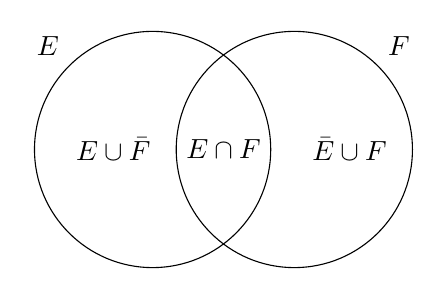
\begin{tikzpicture}
\node [draw,circle,minimum size = 3cm,label={135:$E$}] (E) at (0,0){}; %Set E
\node [draw,circle,minimum size = 3cm,label={45:$F$}] (F) at (1.8,0){}; %Set !F
\node at (0.9,0) {$E \cap F$};
\node at (-0.5,0) {$E \cup \bar F$};
\node at (2.5,0) {$\bar E \cup F$};

\end{tikzpicture}

We can get that $E \cup F = (E \cap \bar F) \cup (E \cap F) \cup (\bar E \cap F)$

So: $P(E \cup F) = P((E \cap \bar F) \cup (E \cap F) \cup (\bar E \cap F))$

Now we use again the third kolmogorov axiom:

$P(E \cup F) = P(E \cap \bar F) + P(E \cap F) + P(\bar E \cap F)$

But now we can transform $P(E \cap \bar F) + P(E \cap F)$ in $P(E)$ 

$P(E \cup F) = P(E) + P(\bar E \cap F)$

We need also $P(F)$, so I add and substract $P(E \cap F)$ which doesn't change anything.

$P(E \cup F) = P(E) + P(\bar E \cap F) + P(E \cap F) - P(E \cap F)$

And so we finished it because the result from getting $P(F)$ is:

$P(E \cup F) = P(E) + P(F) - P(E \cap F)$

Demonstrated.
\bigskip

3. Third theorem

$P(\emptyset) = 0$
\bigskip

Demonstration:

$P(\Omega) = 1$

we know from the first theorem that: $P(\bar E) = 1 - P(E)$

$P(\emptyset) = P(\bar \Omega) = 1 - P(\Omega) = 0$

Demonstrated.

\section{Combination calculus}

Definition: I have a finite set of objects and some ways that allow me to regroup them. I want to count the number of different possible regroups.

\subsection{Principle of enumeration}

I have two experiments. The first with "n" outcomes and the second with "m" outcomes. The sorted couples of possibles outcomes are $n \cdot m$

If I have "n" experiments:

$$m_i = number  \ outcomes \ \ of \ \ i-experiment \longrightarrow m_1 \cdot m_2 \cdot ... \cdot m_n = \prod_{i=1}^n m_i$$

\subsection{Sequencies with repetitions and without repetitions}

I have pinned a certain number of places and I put my objects in queue in these places. The order of the objects does matter.

1. Sequencies with repetitions: let's imagine a rack where we are going to put the objects, we would obtain this kind of situation.

$[n;n;n;n;...;n \ \ \ \ \ ;n \ \ \ \ \ ;]$
 
$\ 1 \ \  2  \ \  3 \ 4 \ \ \ \ \ \ k-1 \  k_{place} $

\bigskip

So:

$$D_{n,k} = n^k$$

2. Sequencies without repetitions: let's imagine the same rack but we can't repeat in this case.

[n;n-1;n-2;...;n-k;n-k+1;]

\bigskip

So:

$$d_{n,k} = \frac{n!}{(n-k)!}$$


\subsection{Permutations}

A unique index. Premutations of "n" objects.

$$P_n = d_{n,n} = n!$$

\subsection{Combinations of n objects on k places}

Same definition of sequencies but the order of objects doesn't matter.

$$C_{n,k} = \frac{d_{n,k}}{k!} = \frac{n!}{k! \cdot (n-k)!} = \left(\begin{array}{c} n \\ k \end{array}\right)$$

\bigskip

The result of the binomial coefficient is the number of possible ways to extract subsets of k elements from a set that contains n elements.

\section{Total probability theorem and Bayes Theorem}

these two theorems can be useful to calculate complex probability by calculating more probabilities that are more simple.

\subsection{Total probability theorem(General form)}

Hypothesis:
\bigskip

A partition of $\Omega \longrightarrow F_1,F_2,...,F_n \subseteq \Omega$ 

$\forall i P(F_i) \neq 0$
\bigskip

Thesis:
$$P(E) = P(\bigcup_{i=1}^n (E \cap F_i)) = \sum_{i=1}^n P(E \cap F_i) = \sum_{i=1}^nP(E|F_i)\cdot P(F_i)$$

Where $P(A|B)$ is a conditional probability defined as follow:

$$P(A|B) = \frac{P(A \cap B)}{P(B)}$$

And from this last definition we say $P(A \cap B) = P(A|B) \cdot P(B)$ 

\subsection{Bayes Theorem}

The hypothesis are the same of the Total probability theorem(General form).
\bigskip

Thesis:

$$P(F_j|E) = \frac{P(F_j \cap E}{P(E)} = \frac{P(E|F_j)\cdot P(F_j)}{\sum_{i=1}^n P(E|F_i) \cdot P(F_i)}$$


From this theorem it's possible to build a classifier that is called Naive Bayes, which allow to simplify the calculus of some probability by using a naive hypothesis. We will not define this classifier here.

\section{Random variable}

A random variable is a function defined as follow:

$$X : \Omega \rightarrow \mathbb{R}$$

Or, if we want to be more precise:

$$\left\{X = \alpha\right\} \equiv \left\{\omega \in \Omega : X(\omega) = \alpha\right\}$$

Basically it's a function that associates a number to each outcome of a random experiment. We define the support as the set of all possible values that a random variable X can assume. 

In this document we will see discreet and continuous random variables.
\bigskip

\subsection{Cumulative Distribution Function}

This function can be defined as the DNA of a random variable, the ID card we can say. It tells us how the variable is distributed.

\bigskip

Definition: $F_x(x) = P(X \leq x)$

Soon we will understand what it means when a random variable is distributed like a certain $F_x$ and we will write $X \sim F_x$. 
\bigskip

Properties of $F_x$:

$F_x : R \rightarrow [0,1]$

$F_x > 0$

$\lim_{x \rightarrow + \infty}F_x(x) = 1$

\subsection{Probability Mass Function}

Only a disreet random variable has this type of function. Discreets random variables assume an enumerable set of specifications. This function is always greater than zero. It's defined as follows:

\bigskip

$p_x : R \rightarrow [0,1]$

$p_x(i) = P(X = i)$

\bigskip

if we do $\sum_{i} p_x(i)$ we obtain 1. Basically we are doing the sum of all specifications that a random variables X can assume, so we are obtaining $\Omega$ and then we are obtaining 1.

\subsection{Probability Density Function}

Only a continous random variable has this type of function. It's defined as follows:

$f_x : R \rightarrow R^+$

\bigskip

$$\forall B \subseteq R, \ P(X \in B) = \int f_x(x)dx$$

$$P(a \leq X \leq b) \int_{a}^{b} f_x(x)dx$$

Now we'll explaining why this can't work using the Probability Mass Function. Basically it would be like calculating: $$P(X = a) = P(a \leq X \leq a) = \int_{a}^{a} f_x(x)dx = 0$$

\bigskip

\bigskip

\bigskip

\bigskip

\bigskip

Properties of a Probability Density Function:

$$First: \ \ \int_{- \infty}^{+ \infty} f_x(x)dx = \int_{R} f_x(x)dx = P(X \in R) = 1$$

$$Second: \ \ \int_{- \infty}^{a} f_x(x)dx = P(X \leq a) = F_x(a) \longrightarrow \frac{d}{dx} F_x(x) = f_x(x)$$

\section{Markov and Tchebyshev inequalities}

These inequalities are interesting theoretic results we can use to give a esteem of a probability.
\bigskip

\subsection{Markov inequality}

Theorem:
\bigskip

$$X \geq 0 \ \ \  \forall a > 0 \rightarrow P(X \geq a) \leq \frac{\mathcal E(X)}{a}$$
\bigskip
Demonstration(For continuous):

$$\mathcal E(X) = \int_{0}^{+ \infty} x \cdot f_x(x)dx = \int_{0}^ax\cdot f_x(x)dx + \int_{a}^{+ \infty} x \cdot f_x(x)dx \geq \int_{a}^{+ \infty} x \cdot f_x(x)dx$$

\bigskip 

$$\geq \int_{a}^{+ \infty} a \cdot f_x(x)dx = a \cdot \int_{a}^{+ \infty} f_x(x)dx = a \cdot P(X \geq a) \longrightarrow \mathcal E(X) \geq a \cdot P(X \geq a)$$

Now we divide both by a and it's demonstrated. The demonstration for discreet variables is almost the same, we use summations instead of integrals.

\subsection{Tchebyshev inequality}

We consider a random variable $X$ with $\mathcal E(X) = \mu$ and $Var(X) = \sigma^2$

Thesis:
$$\forall r > 0 \ \ P(|X - \mu| \geq r) \leq \frac{\sigma^2}{r^2}$$
\bigskip

Demonstration:

$|X - \mu| \geq r \leftrightarrow (X - \mu)^2 \geq r^2$
\bigskip

$P(|X - \mu| \geq r) = P((X - \mu)^2 \geq r^2)$

Let' define $$Y:= (X - \mu)^2 \rightarrow using \ markov \ P(Y \geq r^2) \leq \frac{\mathcal E(Y)}{r^2}$$

$$= \frac{\mathcal E((X- \mu)^2)}{r^2} = \frac{Var(X)}{r^2} = \frac{\sigma^2}{r^2}$$

Demonstrated.

\section{Random variables Models}

Models are useful to solve common problems with a common plan.

\subsection{Bernoulli model}

The bernoulli model describes the most simple experiment such as coin launch and similar. Every experiments have only two outcomes: success or failure.
\bigskip

$X \sim B(p) \ \ \ D_x = \left\{0,1\right\} \ \ \ p \in [0,1]$
\bigskip

$p_x(x) = P(X=x) = p^x \cdot(1-p)^{1-x} \cdot I_\left\{0,1\right\}^{(x)}$

= $1-p$ if $x = 0$ 

= $p$ if $x = 1$

= 0 otherwise
\bigskip

$\mathcal E(X) = p = \sum_{i}x_i P(X=xi)$

$Var(X)=p(1-p)$

\subsection{Binomial model}

This model is obtained from the Bernoulli by doing n bernoulli experiments with the same p parameter and with independence from each other. The variable counts the number of success.

$X \sim B(n,p) D_x = \left\{0,1,...,n\right\}$
\bigskip

$p_x(i) = P(X=i) = \left(\begin{array}{c} n \\ i \end{array} \right) \cdot p^i \cdot (1-p)^{n-i}\cdot I_\left\{D_x\right\}^{(x)}$
\bigskip

$$\mathcal E(X) = \mathcal(\sum_{i=1}^n X_i) = \sum_{i=1}^n \mathcal E(X) = \sum_{i=1}^n p = np$$

$$Var(X) = Var(\sum_{i=1}^n X_i) = \sum_{i=1}^nVar(X_i) = \sum{i=1}^np(1-p) = np(1-p)$$
\bigskip

If we have two binomial indipendent random variables with the same p but different n and we sum them we obtain this:

$$X_1 \sim B(n,p) \ and \ X_2 \sim B(m,p) \rightarrow X_1 + X_2 = Y \sim B(n+m,p)$$


\subsection{Discreet uniform model}

This model is used for experiments such as dice launch.

$X \sim U(n) D_x = \mathbb{N} \cup \left\{0\right\}$

$$p_x(i) = P(X = i) = \frac{1}{n} \cdot I_\left\{1,...,n\right\}^(i)$$
\bigskip

$$\mathcal E(X) = \frac{n+1}{2}$$

$$Var(X) = \frac{n^2 +1}{12}$$

The dispersion around the $\mathcal E(X)$ increase with the number of equal-probability events.


\subsection{Geometric Model}

This model is obtained from the Bernoulli by doing experiments and stop only when it comes the first success. The variable counts the number of failures before the first success. 
\bigskip

$X \sim G(p) \ \ p \in (0,1]$

$p_x(i) = P(X=i) (1-p)^i p \cdot I_{\mathbb{N} \cup {0}^(i)}$
\bigskip

$$\mathcal E(X) = \frac{1-p}{p}$$

$$Var(X) = \frac{1-p}{p^2}$$
\bigskip

This model has the property of Memorylessness that it's defined as follow:

$P(X \geq i + j| X \geq i) = P(X \geq j)$

The number of failures is saying nothing about the next experiment, the probability is the same.

\subsection{Poisson model}

Before talking about the possion model, let's write directly the Probability Mass Function.

$X \sim P(\lambda) D_x = \mathbb{N} \cup \left\{0\right\}$
\bigskip

$$p_x(i) = P(X=i) = e^{- \lambda} \cdot \frac{\lambda^i}{i!} \cdot I_{\mathbb{N} \cup \left\{0\right\}}$$

\bigskip

$\mathcal E(X) = \lambda$

$Var(X) = \lambda$
\bigskip

The really importance of the Poisson model is that we can approximate a Binomial variable with it during certain conditions.
If we have a random variable X distributed as a Binomial with a "big" n and a "little" p (we can say a costant product np), then we can approximate well this variable as a Poisson of parameter $np = \lambda$.
This is possible only when the big n is balanced from a decrease of p.

\bigskip

Demonstration:

$X \sim B(n,p) \ \ \ n \ "big" \ \ \ p \ "little"$

I set $np = \lambda$ with $\lambda > 0 \longrightarrow p = \frac{\lambda}{n}$

$$P(X=i) = \left(\begin{array}{c} n \\ i \end{array} \right) \cdot p^i \cdot (1-p)^{n-i}$$

$$= \left(\begin{array}{c} n \\ i \end{array} \right) \cdot (\frac{\lambda}{n})^i \cdot (1 - \frac{\lambda}{n})^{n-i}$$

$$\frac{n(n-1)...(n-i+1)}{i!} \cdot (\frac{\lambda}{n})^i \cdot (1 - \frac{\lambda}{n})^{n-i}$$

I switch the denominator $i!$ with $n$ and I do a limit for $n \rightarrow + \infty$ 

$$\lim_{n \righarrow + \infty} \left(\frac{n}{n} \cdot \frac{n-1}{n} \cdot ... \cdot \frac{n - i + 1}{n} \cdot \frac{\lambda^i}{i!} \cdot \frac{(1 - \frac{\lambda}{n})^n}{(1 - \frac{\lambda}{n})^i}\right)$$

the first part tends to 1, the fraction with $\lambda$ doesnt depend from n and we ignore it, we have to determine the last one:
\bigskip

we know that: $$\lim_{n \rightarrow + \infty} (1 + \frac{1}{n})^n \rightarrow e^1$$

So the numerator tends to $e^{- \lambda}$ and the denominator tends to 1.

The result of the limit is: $$\frac{\lambda^i}{i!} \cdot e^{- \lambda}$$

This is literally the probablity mass function of a poisson random variable, so it's demonstrated.

\subsection{Exponential model}

This model is used for the time that pass between two events in the case the events exist based of some hypothesis.

$X \sim E(\lambda) \lambda \in R^+$
\bigskip

$f_x(x) = \lambda \cdot e^{- \lambda x} \cdot I_\left\{R^+\right\}^(x)$
\bigskip

$\mathcal E(X) = \frac{1}{\lambda}$

$Var(X) = \frac{1}{\lambda^2}$
\bigskip


The exponential model has something in common with the Geometric one, such as the Probability mass function graph of the geometric with the probability density function graph of the exponential. Both models has the Memorylessness property.
\bigskip

Demonstration:

$$F_x(x) = 1 - e^{-\lambda x} \rightarrow P(X > x) = 1 - F_x(x) = e^{- \lambda x}$$

$$P(X > s + t) = e^{- \lambda (s+t)} = e^{-\lambda s} \cdot e^{- \lambda t}$$

$$P(X > s + t ) = P(X > s)P(X > t)$$

$$P(X>s) = \frac{P(X > s +t )}{P(X > t)} \rightarrow Memorylessness \frac{P(X > s \cap X > t)}{p(X > t)}$$

And so: $P(X > s + t | x > t) = P(X>s)$

Demonstrated.

\section{The Gaussian/Normal model}

$X \sim G(\mu,\sigma) \ \ \mu \in R \ \ \ \sigma \in R^+$

$$f_x(x) = \frac{1}{\sqrt{2\pi}\sigma}\cdot e^{\frac{- (x - \mu)^2}{2\sigma^2}}$$

There's no need of a index set because $D_x$ is defined on all R.

\bigskip

$\mathcal E(X) = \mu$

$Var(X) = \sigma^2$

\bigskip

If I calculate $aX +b:= Y$ 

$X \sim G(\mu,\sigma) \rightarrow Y \sim G(aX +b,\sigma)$

\bigskip

If I consider two gaussian variables with independence:

$X_1 \sim G(\mu_1,\sigma_1)$ and $X_2 \sim G(\mu_2,\sigma_2)$

$X_1 + X_2 \sim G(\mu_1+\mu_2,\sqrt{\sigma_1^2 + \sigma_2^2})$

\subsection{Standardization}

The standardization is defined as follow:

$$Y = \frac{X - \mu}{\sigma}$$

The result is again a Gaussian variable with $\mathcal E(X) = 0$ and $Var(X) = 1$.

This type of gaussian has a particolar name: standard normal.

$X \sim N(0,1)$

\bigskip

summarizing the Standard Normal:

$$Z:= \frac{X -\mu}{\sigma} \sim N(0,1)$$

$$P(Z > x) = 1 - P(Z \leq x) = 1 - \Phi(x)$$

\subsection{Reproduction}

If we have $X_1,...,X_n$ gaussian variables with independence $$X_i \sim G(\mu_i,\sigma_i)$$

we define $$Y = \sum_{i=1}^n X_i \longrightarrow \mathcal E(Y) = \sum_{i=1}^n\mu_i \ \ \ Var(Y) = \sum_{i=1}^n \sigma_i^2$$

$$Y \sim G\left(\sum_{i=1}^n \mu_i, \sqrt{\sum_{i=1}^n \sigma_i^2}\right)$$

This behavior is similar to what we have seen with the binomial variable.

The Poisson model has this exact property too.

\section{Central Limit Theorem}

Hypothesis:

$X_1,...,X_n$ random variables with independence and with same distribution

$\forall i \ \ \ \mathcal E(X_i) = \mu \ \ \ Var(X_i) = \sigma^2$

\bigskip

If I sum all of these variables I can say:

$$\sum_{i=1}^n X_i \dot \sim N(n\mu,\sqrt{n}\sigma)$$

\bigskip

\bigskip

And if I do the standardization:

$$\frac{\sum_{i=1}^n X_i - n\mu}{\sqrt{n}\sigma} \dot \sim N(0,1)$$

This approximation is better when the number of random variables is high(our n).

Now, if we want to be more formal:

$$\lim_{n \rightarrow +\infty} P\left(\frac{\sum_{i=1}^n X_i - n\mu}{\sqrt{n} \sigma} \leq x\right) = \Phi(x)$$

Where $\Phi(x)$ is the cumulative ditribution function of the Standard Normal.

\section{Law of larger number}

This is the only notion of Inferential statistic parametric you will read in this document. There are other concepts that you can read on the Jupyter Notebook.

This law has two forms: strong and weak.

\bigskip

The strong one:

$$P\left(\lim_{n \rightarrow + \infty} \bar X_n =\mu\right) = 1$$

More the number of elements in the sample we have, less the $\bar X$ is a random quantity, it becomes a constant which is exactly what I want to esteem.


\bigskip

The weak one:

$$\lim_{n \rightarrow + \infty} P\left(|\bar X_n - \mu| > \epsilon\right) = 0$$

I pin an epsilon that tell me when the error is too much. This is the probability that the error in the esteem is too much and with n that tends to infinity this probability tends to zero $\forall \epsilon > 0$.

\section{Poisson Process}

Poisson process is a stochastic process that can be used to gain interesting results. For example if we have data of many events where the event is: "They called me for advertising", it's possible to predict the exact time of the next phone call with this tool.

\bigskip

Let's define a few actors: 

$t = 0$ instants of time.

$N(t): \ \ random \ \ variable \rightarrow N(t)$ are the events that happen in $[0,t]$

\bigskip

N that varies of "t" is a stochastic process. A stochastic process is a process characterized from events that have a probability which have sense only for small intervals.

As t varies, I have a family of random variables.

\bigskip

There are 4 hypothesis to use the Poisson Process:

1. $N(0) = 0$ which meeans the time 0, before that it happens nothing.

2. Independence of disjoint intervals. 

3. $$\lim_{h \rightarrow 0} \frac{P(N(\lambda) = 1)}{h} = \lambda$$

\bigskip

This third hypothesis is saying that more "h" is near to 0, more the fraction can be well approximed by $\lambda$.

\bigskip

More formal: $\exists \lambda : \lim_{h \rightarrow 0} = \lambda$

If I consider small intervals starting from zero, the probability that there's an exact event that happen in this interval depends from the length of the interval.

\bigskip

more formal: $h \ \ is \ \ small \longrightarrow P(N(\lambda) = 1) \approx \lambda \cdot h$

4. $$\lim_{h \rightarrow 0} \frac{P(N(\lambda) \geq 2}{h} = 0$$

The fourth hypothesis says that if I have a small "h", the probability of getting 2 or more events is approximed to zero.

\bigskip

\bigskip

If these 4 hypothesis exists then:

$$N(t) \sim P(\lambda \cdot t)$$

So: $$P(N(t) = k) = e^{- \lambda t} \cdot \frac{(\lambda t)}{k!} \cdot I_{N \cup \left\{0\right\}^{(k)}$$

That probability explained: I have exactly k events happened on a interval between 0 and t. It doesn't matter if I start from zero, it works even if I start from a "s" value.

$$P(X_1 > t) = P(N(t) = 0) = e^{\lambda t} \cdot \frac{(\lambda t)^0}{0!} = e^{- \lambda t}$$

$$F_{x_1}(t) = P(X_1 \leq t) = 1 - P(X_1 > t) = 1 - e^{- \lambda t} \longrightarrow X_1 \sim E(\lambda)$$

Using the memorylessness property of the exponential model, you can demonstrate that: $$\forall i \ X_i \sim E(\lambda) i.i.d.$$

\bigskip

\bigskip

Conclusions: If exists the hypothesis of Poisson Process...

\bigskip

1. The number of occurences of events in a interval of lenght "t" is well described by a Poisson model of parameter $\lambda t$.

2. The time that passes between two events is distributed as an exponential of parameter $\lambda$.

\section{Conclusion}

Other concepts will be inside the jupyter notebook I put in this repository.
I ignored many details such as the demonstration of how some $\mathcal E(X)$ and $Var(X)$ have those values and why.

\end{document}
